\chapter{Modelowanie wielowymiarowych zmiennych losowych}

W tym rozdziale rozważymy \textit{n}-wymiarowe wektory losowe $\mathbf{X} = [X_1, X_2, \dots, X_n]$ i połączymy klasyczne, probabilistyczne podejście do opisu ich rozkładów z teorią kopuł, zapoczątkowaną w \cite{Sklar_Theorem}.\\
Ten rozdział zbudowany jest następująco: w \ref{sec:rozklady_laczne} przypomnimy elementy rachunku prawdopobieństwa pozwalające nam opisać czym są kopuły. Definiujemy je następnie dla przypadku dwuwymiarowego w \ref{sec:dwuwymiarowe_kopuly}, oraz rozszerzamy definicję na przypadek wielowymiarowy w \ref{sec:kopuly_w_wyzszych_wymiarach}. Rozdział \ref{sec:kopuly_w_wyzszych_wymiarach} omawia również techniczny problem konstrukcji takich kopuł, porównując konkurujące w praktyce podejścia: analityczne i Vine Copula.\\

\section{Zmienne losowe i rozkłady łączne}
\label{sec:rozklady_laczne}
Rozpatrywać będziemy przestrzeń probabilistyczną $(\Omega,\mathcal{F},P)$, czyli niech $\Omega$ to pewien niepusty zbiór, $\mathcal{F}$ to $\sigma$-ciało zdarzeń losowych, a $P$ to funkcja $P\colon\Omega\rightarrow[0,1]$. 

\begin{df}[\textit{n}-wymiarowa zmienna losowa]\cite{Rachunek_prob}
	\label{df:n_wym_zmienna_losowa}
	\textit{n}-wymiarową zmienną losową nazywamy funkcję określoną na przestrzeni zdarzeń elementarnych $\Omega$ i przyjmującą wartości rzeczywiste:
	
	$$ X\colon \Omega \mapsto \mathbb{R}^{n}, $$

	taką, że
	
	$$ \{ \omega \colon X(\omega) < x) \} \in \mathcal{F},$$
	
	dla każdego $x \in \mathbb{R}.$
\end{df}


\subsection{Narzędzia opisu zmiennych losowych}
Zmienna losowa jest matematycznym modelem nieznanej, losowej wielkości. Jest ona jednoznacznie opisywana przez dystrybuantę - mówiącą nam z jakim prawdopodobieństwem zmienna może występować w konkretnych obszarach swojego zbioru wartości.

\begin{df}[Dystrybuanta]\cite{Rachunek_prob}
	Dystrybuantą wektora losowego $\mathbf{X} = [X_1, X_2, \dots, X_n]$ nazywamy funkcję:
	$$
	F_{\mathbf{X}}(x_1, \dots, x_n)=P(X_1 < x_1, \dots, X_n < x_n).
	$$
\end{df}

W tej pracy skupiamy się jedynie na zmiennych losowych typu ciągłego, czyli takich których dystrybuanta daje się przedstawić w postaci $ F_{\mathbf{X}}(x) =\int_{-\infty}^{x}f_{\mathbf{X}}(s) ds$ dla pewnej nieujemnej funkcji $f_{\mathbf{X}(s)}$ nazywanej funkcją gęstości rozkładu. Gęstość, jeżeli jest określona, również może być użyta do jednoznacznej identyfikacji zmiennej losowej.\\

Do opisu najpopularniejszych jednowymiarowych rozkładów dostępne mamy zazwyczaj analityczną postać ich dystrybuanty lub gęstości. Ponieważ literatura podaje różne ich parametryzacje, w tabeli \ref{tab:przykladowe_zmienne_losowe} podajemy gęstości zmiennych losowych przewijających się w tej pracy. Ich wykresy widoczne są na wykresie \ref{fig:przykladowe_zmienne_losowe}. Przykłady wielowymiarowych dystrybuant i gęstości podamy w rozdziale \ref{subsec:rozklady_wielowymiarowe}. 

Warto wspomnieć, że istnieją również użyteczne rozkłady, które nie dają się wyrazić za pomocą gęstości czy dystrybuanty. Najpopularniejszym przykładem mogą być rozkłady stabilne, które w ogólności nie posiadają dystrybuanty jawnej postaci i musimy posługiwać się zamiast tego ich funkcją charakterystyczną. \cite{Stable_Distributions1}, czy \cite{Stable_Distributions2} podają bardzo dobry przegląd teorii rozkładów stabilnych i pokazują ich przewagę w kontekście modelowania nie-gaussowskich zwrotów na rynkach finansowych. \cite{LevyFlights} pokazują natomiast, że modele procesów stochastycznych oparte o rozkład Levy'ego (tzw. \textit{Levy flights}) dobrze nadają się do opisu dynamiki wskaźników finansowych powszechnie używanych w raportach spółek.

\begin{table}[h]
	\caption{\textbf{Popularne zmienne losowe.} Tabela przedstawia dystrybuanty, oraz gęstości popularnych jednowymiarowych zmiennych losowych pojawiających się w tej pracy.}
	\label{tab:przykladowe_zmienne_losowe}
	\begin{tabular}{ll|c|c}
		\hline
		\textbf{Rozkład} & \textbf{Oznaczenie} & \textbf{Nośnik} & \textbf{Gęstość} \\
		\hline
		Normalny & $\mathcal{N}(\mu, \sigma)$ & $\mathbb{R}$ & $\frac{1}{\sigma \sqrt{2 \pi}} \exp\big(-\frac{(x-\mu)^2}{2\sigma^2}\big)$\\ 
		T-studenta & $\text{t}(\mu, \sigma, \nu)$ & $\mathbb{R}$ & $ \frac{\Gamma(\frac{\nu + 1}{2})}{\Gamma(\frac{\nu}{2})\sqrt{\pi\nu}\sigma} \bigg[1 + \big(\frac{x - \mu}{\sigma}\big)^2\frac{1}{\nu}\bigg]^{-\frac{\nu + 1}{2}} $ \\ 
		Beta & $\text{Beta}(\alpha, \beta)$ & $[0, 1]$ & $ x^{\alpha - 1}(1 - x)^{\beta - 1}\frac{\Gamma(\alpha + \beta)}{\Gamma(\alpha)\Gamma(\beta)}$ \\ 
		Wykładniczy & $\text{Exp}(\lambda)$ & $\mathbb{R}^{+}$ & $ \lambda e^{-\lambda x}$ \\
		Gamma & $\mathcal{G}(\alpha, \beta)$ & $\mathbb{R}^+$ & $x^{\alpha - 1}e^{-\beta x}\frac{\beta^\alpha}{\Gamma(\alpha)}$\\ 
		
		\hline
	\end{tabular}
\end{table}

\begin{figure}[H]
	\centering
	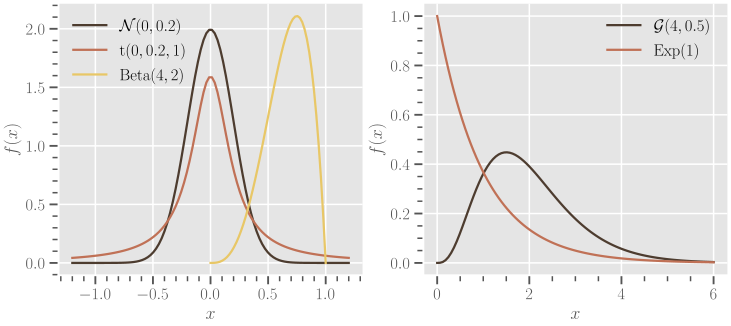
\includegraphics[width=\linewidth]{01_Rozklady_1D}
	\caption{Przykładowe gęstości zmiennych losowych z tabeli \ref{tab:przykladowe_zmienne_losowe}.\label{fig:przykladowe_zmienne_losowe}}
\end{figure}

\subsection{Rozkłady wielowymiarowe}

W klasycznym studium doboru struktury portfela przedstawionym w \cite{Markovitz_MPT}, Markovitz analizuje portfel aktywów. Przedmiotem tej pracy jest opis sposobu, w jaki indywidualne pozycje w portfelu wpływają na jego całościowy zwrot i ryzyko. Współczesna teoria portfela która została zapoczątkowana tą pracą wymaga zamodelowania całego systemu jakim jest zbiór akcji w portfelu. Markovitz pokazuje w swojej pracy istotę współzależności między poszczególnymi aktywami, od której zależy czy ryzyko portfela ulega dywersyfikacji, czy jest amplifikowane. Modelowanie każdego aktywa z osobna jest niewystarczające, ponieważ istota ich wpływu na portfel tkwi w przeważającym stopniu we współzależnościach pomiędzy nimi.\\
Naturalnym jest więc, że w praktyce rozważamy modele wielowymiarowych zmiennych losowych, które mają w sobie zakodowane współzależności i pozwalają przez to lepiej uchwycić losową naturę zjawiska. Z tego samego powodu jednak, rozkłady wielowymiarowe są dużo trudniejsze do modelowania niż ich jednowymiarowe odpowiedniki. Nie wystarczy bowiem zamodelować rozkładów konkretnych współrzędnych wielowymiarowego wektora, lecz należy dodatkowo określić w jaki sposób rozkład tej zmiennej będzie wyglądał, gdy pozostałe zmienne przyjmą wartości w pewnym zbiorze. Odpowiedzi na te pytania dostarczają nam gęstości brzegowe i warunkowe wielowymiarowego rozkładu.
\begin{df}[Rozkłady brzegowy]
	Rozpatrzmy d-wymiarową zmienną losową $\mathbf{X} = [X_1, X_2, \dots, X_d]$ o gęstości $f(x_1, \dots, x_d)$. Gęstość rozkładu brzegowego $f_{j}(x_j)$ definiujemy jako:
	$$f_j(x_j)=\int_{-\infty}^{\infty}\dots\int_{-\infty}^{\infty} f(x_1, \dots, x_{j-1}, x, x_{j+1}, \dots, x_d)  dx_1\dots dx_{j-1} dx_{j+1} \dots dx_d.$$
\end{df}

\begin{df}[Rozkład warunkowy]
	Rozpatrzmy d-wymiarową zmienną losową $\mathbf{X} = [X_1, X_2, \dots, X_d]$ o gęstości $f(x_1, \dots, x_d)$. Gęstość rozkładu warunkowego definiujemy jako:
	 $$f_{j|k}(x_j|x_k) = \frac{f(x_1, \dots, x_d)}{f_k(x_k)}.$$
\end{df}

Rozkłady jednowymiarowe z tabeli \ref{tab:przykladowe_zmienne_losowe} w naturalny sposób znajdują swoje rozszerzenia na więcej wymiarów (\cite{MultivariateDistributions}, \cite{Cherubini_Copula_Methods_in_Finance}). Najpopularniejszym tego przykładem jest rodzina $d$-wymiarowych rozkładów eliptycznych, do której należą rozkłady o gęstości postaci:

$$ f_{\mathcal{N}}(x, \mu, \Sigma) = k_d \vert\Sigma\vert^{-0.5}g\big((x-\mu)^T\Sigma^{-1}(x-\mu)\big).$$

W powyższej reprezentacji, $k_d \in\mathbb{R}$ jest stałą zależną od wymiaru, $\mu$ jest $d$-wymiarowym wektorem średnich, $\Sigma \in \mathbb{R}^{d \times d}$ to symetryczna, dodatnio zdefiniowana macierz, a $g \colon [0, \infty) \mapsto [0, \infty)$ jest pewną funkcją która nie zależy od wymiaru wektora.

Dla odpowiednio dobranych $g$ i $k_d$ otrzymamy w tej rodzinie wielowymiarowy rozkład normalny, czy wielowymiarowy rozkład t. Powstają one przy odpowiednio $k_d=(2\pi)^{-0.5d}$ i $g(s) = \exp(-0.5 t)$, lub $k_d=\Gamma(\frac{\nu + d}{2})/\Gamma(\frac{\nu}{2})$ i $g(s) = \big(1 + \frac{t}{\nu})^{-(\nu + d)/2}$.
\begin{figure}[H]
	\centering
	\includegraphics[width=0.45\linewidth]{01_MultivariateGaussian}	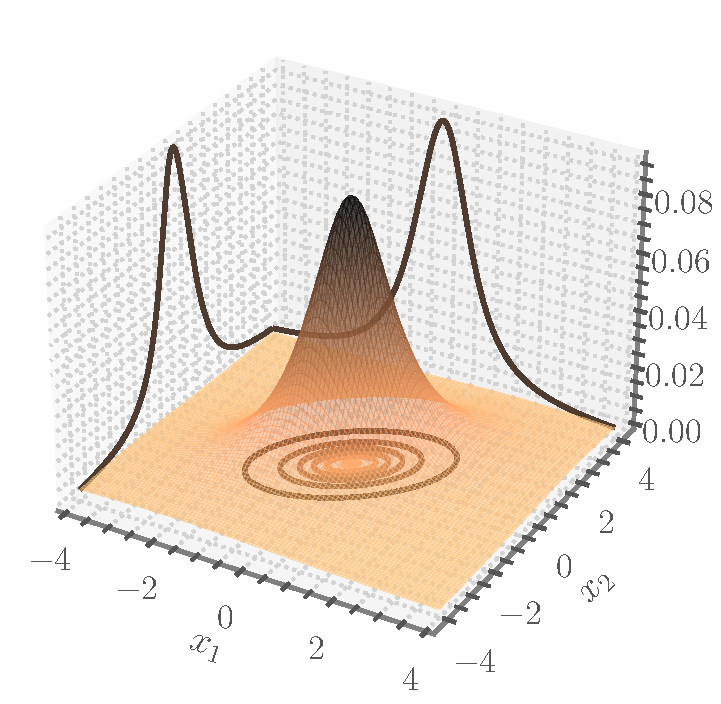
\includegraphics[width=0.45\linewidth]{01_MultivariateStudent}
	\caption{Gęstości przykładowych rozkładów eliptycznych ($d=2, \mu=[0, 0], \Sigma = \big[\begin{smallmatrix}2&1\\1&2\end{smallmatrix}\big]$). Lewy panel: $2$-wymiarowy rozkład normalny. Prawy panel: $2$-wymiarowy rozkład t ($\nu = 0.5$).\label{fig:multivariate_gaussian_student}}
\end{figure}

Obserwując rysunek \ref{fig:multivariate_gaussian_student}, można rozpoznać charakterystyczne kształty rozkładów brzegowych. Przy wielowymiarowym rozkładzie normalnym obserwujemy gaussowski dzwon, a dla wielowymiarowego rozkładu $t$ otrzymujemy ciężkoogonowe rozkłady brzegowe $t$-studenta. Używając rozkładów eliptycznych, implikujemy bowiem model w którym rozkłady brzegowe pochodzą z tej samej rodziny. Manipulując różnymi rozkładami eliptycznymi możemy więc zamodelować szeroką gamę korelacji między zmiennymi, czy też ciężkie ogony, zachowując prostotę i analityczną postać modelu. Tracimy jednak swobodę wyboru rozkładów brzegowych. \cite{Markovitz_MPT} i jego model bazują na rozkładzie multinormalnym, zakładając że wektor średnich i macierz korelacji wystarczająco opisuje rozkład zwrotów aktywów rynkowych. Można to uznać za nierealistyczne i oderwane od rzeczywistości ze względu na empiryczne dowody ciężkoogonowego charakter zwrótów na rynku akcji \cite{Mandelbrot_NonGaussianity}, czy zjawiska silniejszej korelacji w lewym ogonie \cite{Kurowicka_Dependence_Modeling}. Nie mniej jednak nie da się odmówić, że ten prosty model jest wystarczający aby zilustrować jak istotny jest wpływ zależności komponentów na zachowanie całego systemu. \\
Na szczęście dzięki \cite{Sklar_Theorem}, dostepne mamy narzędzia pozwalające uchwycić te zależności dużo dokładniej i \cite{Cherubini_Copula_Methods_in_Finance} czy \cite{Kurowicka_Dependence_Modeling} słusznie wymieniają wiele realnych przykładów gdzie taki wyższy poziom elastyczności modelu jest niezastąpiony. Kolejny rozdział rozpoczniemy od jednego z takich przykładów, w celu umotywowania popularności modeli kopułowych jako odpowiedzi na te potrzeby.

\section{Dwuwymiarowe kopuły}
\label{sec:dwuwymiarowe_kopuly}
\subsection{Wprowadzenie i definicja}
Teorię kopuł zapoczątkował Abe Sklar w \cite{Sklar_Theorem}, podając następujące twierdzenie:

\begin{thm}[Twierdzenie Sklara]
	Niech $X_1, X_2, \dots, X_d$ będą zmiennymi losowymi ciągłymi, o dystrybuantach $F_1, \dots, F_d$, i rozkładzie łącznym z dystrybuantą $F$. Wtedy istnieje unikalna \emph{kopuła} $C$, taka że dla wszystkich $\mathbf{x} = (x_1, \dots, x_d) \in \mathbb{R}^n$:
	\begin{equation}
		F(x_1, \dots, x_d) = C(F_1(x_1), \dots, F_d(x_d)).
		\label{eq:sklar_theorem}
	\end{equation}
	
	Zachodzi również twierdzenie odwrotne: Mając dowolne dystrybuanty $F_1, \dots, F_d$ i kopułę $C$, funkcja $F$ zdefiniowana według \ref{eq:sklar_theorem} jest d-wymiarową dystrybuantą, o rozkładach brzegowych $F_1, \dots, F_d$. 
	\label{thm:sklar_theorem}
\end{thm}

Twierdzenie \ref{thm:sklar_theorem} przede wszystkim podaje więc algorytm postępowania mówiący w jaki sposób otrzymać wielowymiarowy rozkład o dowolnie wybranych, potencjalnie różnych rozkładach brzegowych. Dodatkowo, Sklar stwierdza istnienie pewnego obiektu, nazwanego kopułą/funkcją łączącą (łac.\emph{copulae}: łączyć) który jest jednoznacznie zdefiniowany dla dowolnego ciągłego rozkładu wielowymiarowego, w taki sposób, że rozkład łączny da się przedstawić jako tę funkcję zaaplikowaną do rozkładów brzegowych.\\

Oczywistym jest, że nie wszystkie wielowymiarowe funkcje mogą pełnić taką rolę. Rozważymy więc jakie warunki musi spełniać $C$ z twierdzenia \ref{thm:sklar_theorem}, aby mogła być kopułą.
\begin{df}[Grounded function]
	Rozważmy $A_1$ i $A_2$ - dwa niepuste podzbiory $\mathbb{R}$, oraz funkcję $G\colon A_1\times A_2\mapsto\mathbb{R}$. Niech $a_i$ oznacza najmniejszy element $A_i$, dla $i=1, 2$. Funkcję $G$ będziemy nazywać uziemioną \emph{(eng. grounded)}, jeśli dla każdej pary $(v, z)$ z $A_1\times A_2$,
	\begin{equation}
		G(a_1, z) = 0 = G(v, a_2).
	\end{equation}
	\label{def:grounded_function}
\end{df}

\begin{df}[2-increasing function]
	$G\colon A_1\times A_2\mapsto \mathbb{R}$ nazywamy dwu-rosnącą \emph{(eng. 2-increasing)}, jesli dla każdego prostokąta $[v_1, v_2]\times [z_1, z_2]$ $(v_1 \leqslant v_2$, $z_1\leqslant z_2)$ którego wierzchołki leżą w $A_1 \times A_2$ mamy
	\begin{equation}
		G(v_2, z_2) - G(v_2, z_1) - G(v_1, z_2) + G(v_1, z_1) \geqslant 0.
	\end{equation}
	\label{def:two_increasing_function}
\end{df}

Definicje \ref{def:grounded_function} oraz \ref{def:two_increasing_function} pozwalają na poprawne zdefiniowanie kopuły:
\begin{df}[Dwuwymiarowa kopuła]
	Dwuwymiarową kopułą $C$ nazwiemy funkcję rzeczywistą zdefiniowaną na kwadracie jednostkowym:
	$$ C\colon [0, 1]\times[0, 1] \mapsto \mathbb{R},$$ o następujących własnościach:
	\begin{itemize}
		\item uziemiona $\big(C(v, 0) = 0 = C(0, z)\big)$
		\item dwu-rosnąca
		\item $C(v, 1) = v$ oraz $C(1, z) = z$ dla wszystkich $(v, z)\in [0,1]\times [0, 1].$
	\end{itemize}
	\label{def:bivariate_copula}
\end{df}

Aby zrozumieć czym kopuła tak naprawdę jest warto wrócić do twierdzenia \ref{thm:sklar_theorem}. Równość \ref{eq:sklar_theorem} implikuje, że kopuła musi być dystrybuantą pewnego wielowymiarowego rozkładu. Definicję kopuły w \ref{def:bivariate_copula} mówi natomiast widzimy, że ta dystrybuanta jest zdefiniowana na \emph{kwadracie jednostkowym}. Kopułą jest więc niczym innym jak dystrybuantą wielowymiarowego rozkładu jednostajnego. Istotnie: można pokazać, że argumenty kopuli w równaniu \ref{eq:sklar_theorem} mają rozkład jednostajny, co udowadniamy poniżej i ilustrujemy na rysunku \ref{fig:PIT}.

\begin{df}[Probability integral transform]
	Jeśli $X\sim F$ jest ciągłą zmienną losową, a $x$ jest jej realizacją, to transformację $u\coloneqq F(x)$ nazywamy \emph{probability integral transform} (PIT) w punkcie $x$.
\end{df}
\begin{thm}[Probability integral transform]
	Jeśli $X\sim F$ jest ciągłą zmienną losową, to $U\coloneqq F(X)$ ma rozkład jednostajny.
\end{thm}
\begin{proof}
	$$P(U\leqslant u) = P(F(X) \leqslant u) = P(X\leqslant F^{-1}(u))=F(F^{-1}(u))=u.$$
\end{proof}

\begin{figure}[H]
	\centering
	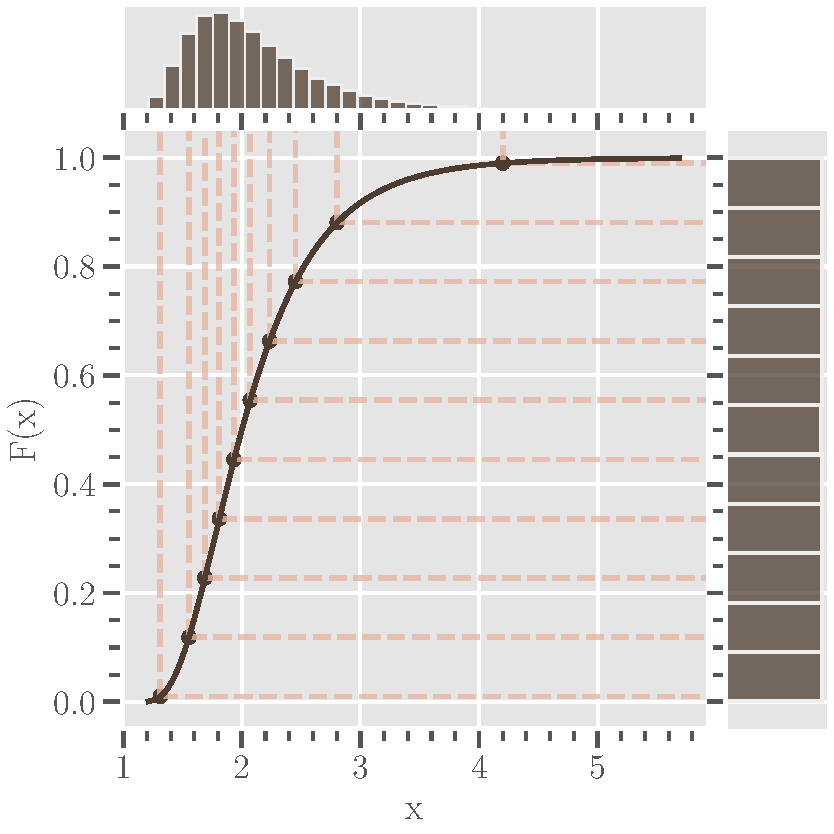
\includegraphics[width=0.6\linewidth]{01_PIT}	
	\caption{Ilustracja działania PIT. Zmienna losowa z rozkładu $
		\mathcal{LN}(0.5, 1)$ (pozioma oś) przekształcana jest przez własną dystrybuantę do rozkładu jednostajnego $\mathcal{U}(0, 1)$ (pionowa oś).\label{fig:PIT}}
\end{figure}

Wróćmy na chwilę do oryginalnego pytania, czyli modelowania wielowymiarowych zmiennych losowych. Na początku rozdziału zdefiniowaliśmy kopułę jako funkcję spełniającą równanie \ref{eq:sklar_theorem} z twierdzenia Sklara, czyli:
$$F(x_1, \dots, x_d) = C(F_1(x_1), \dots, F_d(x_d)).$$

Prawą stronę równania stanowią wyizolowane rozkłady brzegowe, oraz pewna funkcja $C$, postać której jest kompletnie od nich niezależna. Lewa strona równania, to natomiast rozkład łączny pewnej zmiennej losowej. Jeśli zastanowimy się co wpływa na charakter rozkładu łącznego zmiennej losowej, dojdziemy do wniosku, że istnieją dwa komponenty: zachowanie rozkładów brzegowych, oraz ich współzależności. Biorąc znów pod uwagę prawą stronę równania, kopuła musi więc odpowiadać za współzależności między rozkładami brzegowymi. \\
Istotnie, kopuły pozwalają na rozdzielenie problemu modelowania rozkładu łącznego, na modelowanie osobno rozkładów brzegowych, a osobno struktury ich współzależności (\cite{Sklar_Theorem}, \cite{Joe_Multivariate_Models}). Ta pozorna prostota tworzenia wielowymiarowych modeli przyczyniła się do szybkiej ich popularyzacji, ale i przyniosła ze sobą duże ryzyko modelu. Najbardziej znanym tego przykładem jest zapewne fiasko modeli wyceniających produkty typu CDO (\cite{CDS_Copula}), które niedoszacowywały nasilenia korelacji bankructw wewnątrz struktury tego kontraktu.\\

Zauważamy zatem dualizm kopuł - można patrzeć na nie zarówno jak na funkcje łączące ze sobą dowolne rozkłady brzegowe w spójny rozkład łączny, lub też jak na dystrybuanty wielowymiarowych rozkładów jednostajnych.\\
\label{subsec:dwuwymiarowe_kopuly_definicja}

\subsection{Probabilistyczna interpretacja}
Przyjrzymy się więc jednej stronie powyższego dualizmu i przeanalizujmy kopuły jako struktury zależności.

\begin{df}[Kopuła minimum]
	Dwuwymiarowa kopuła minimum $C^{-}$ to kopuła zadana wzorem $C^{-}(u, v) = \max(u+v-1, 0).$
\end{df}
\begin{df}[Kopuła maximum]
	Dwuwymiarowa kopuła maksimum $C^{+}$, to kopuła zadana wzorem $C^{+}(u, v) = \min(u, v).$
\end{df}

\begin{figure}[h]
	\centering
	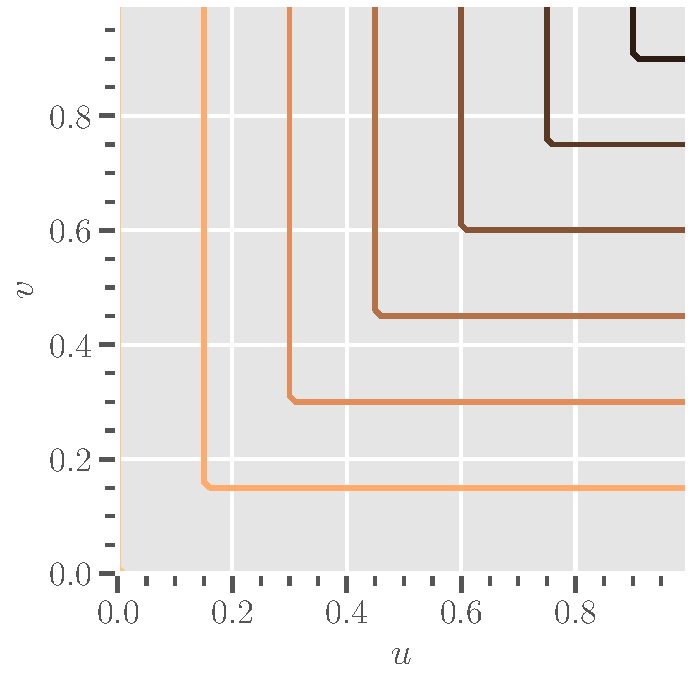
\includegraphics[width=0.35\linewidth]{01_MaximumCopula_contour}
	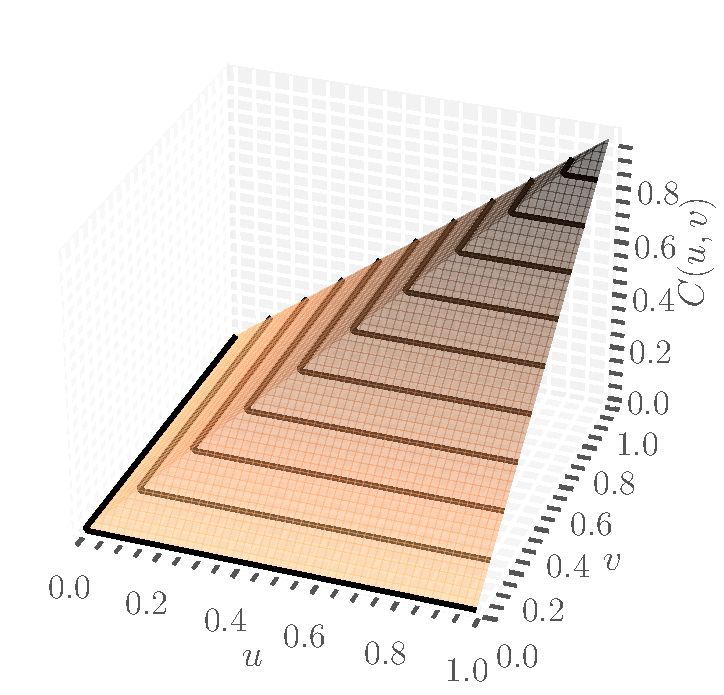
\includegraphics[width=0.4\linewidth]{01_MaximumCopula_surface}
	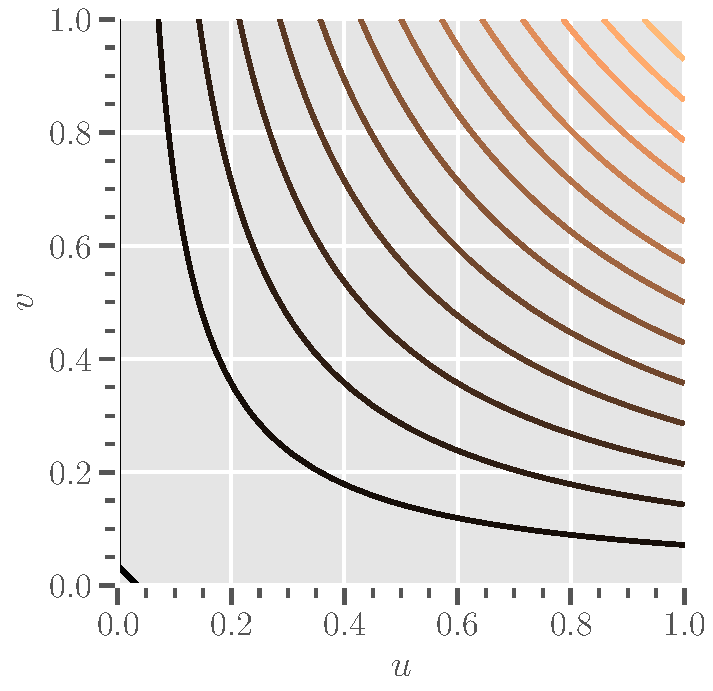
\includegraphics[width=0.35\linewidth]{01_IndependenceCopula_contour}
	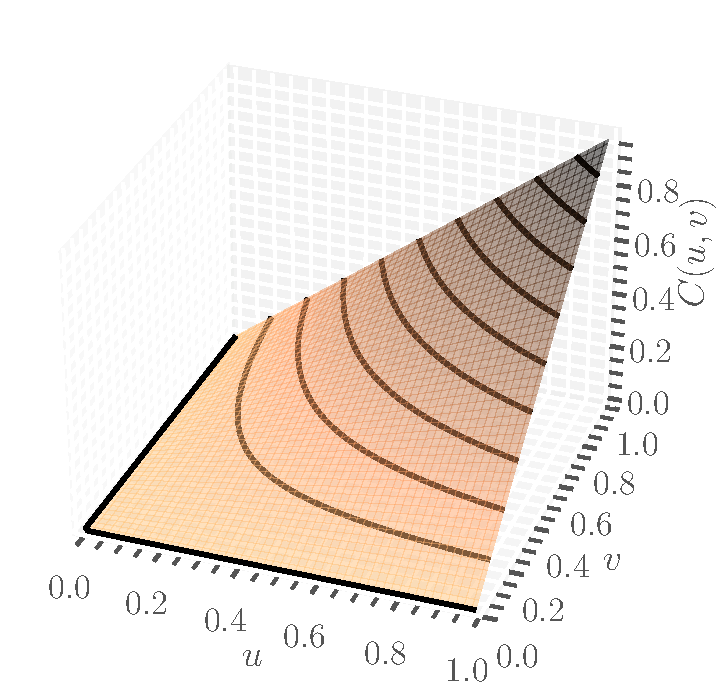
\includegraphics[width=0.4\linewidth]{01_IndependenceCopula_surface}
	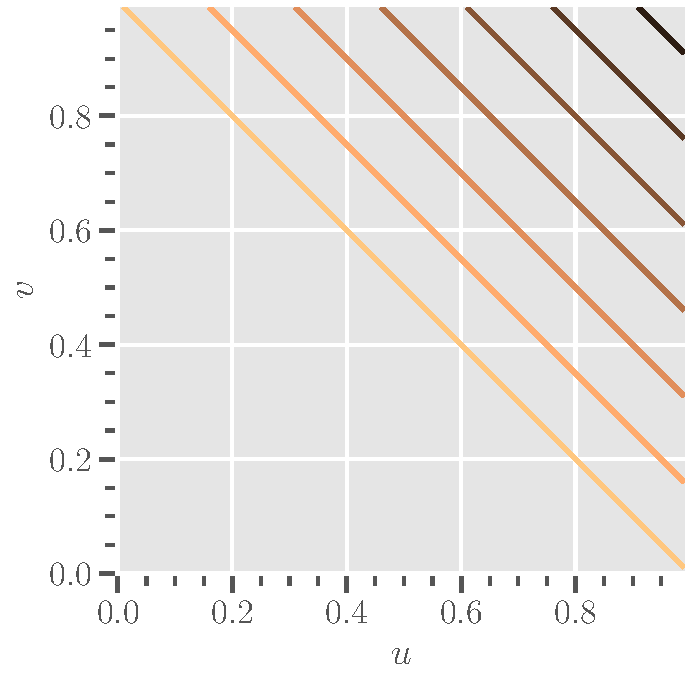
\includegraphics[width=0.35\linewidth]{01_MinimumCopula_contour}
	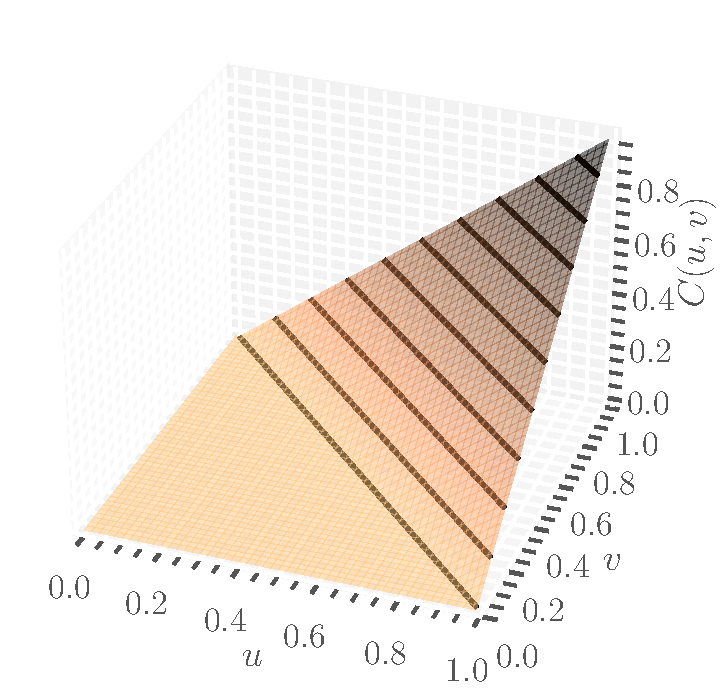
\includegraphics[width=0.4\linewidth]{01_MinimumCopula_surface}
	
	\caption{Dystrybuanty (po lewej) i kontury (po prawej) kopuł: maximum (górny panel), produktowej (panel środkowy) i minimum (dolny panel)\label{fig:minmaxprod_copula}}
\end{figure}

Powyższe kopuły stanowią horyzont osiągalnych kopuł, ponieważ jak mówi twierdzenie \ref{thm:frechet_hoeffding}, są one ograniczeniem dolnym i górnym dla dowolnej innej kopuli. Ich powierzchnie i kontury przedstawia rysunek \ref{fig:minmaxprod_copula}. 

\begin{thm}[Fréchet-Hoeffding bounds]
	Niech $C$ będzie $2$-wymiarową kopułą. Wtedy dla każdego $(u, v)\in[0, 1]^2$ zachodzi
	
	$$ C^{-}(u, v) \leqslant C(u, v) \leqslant C^{+}(u, v).$$
	
	\label{thm:frechet_hoeffding}
\end{thm}

Twierdzenie to, choć z pozoru teoretyczne, ciągnie za sobą bardzo praktyczne konsekwencje: pozwala otrzymać niezależne od modelu ogranicznia górne i dolne na dowolną kopułę. \cite{Cherubini_Copula_Methods_in_Finance} pokazuje przykład, gdzie twierdzenie Frécheta-Hoeffdinga pozwala na uzyskanie dolnego i górnego ograniczenia na pewne statystyki modelu, jak np. łączne prawdopodobieństwo bankructwa dwóch firm w strukturalnym modelu Mertona, czy cena opcji binarnej na dwa aktywa.

\begin{df}[Kopuła produktowa]
	Dwuwymiarowa kopuła produktowa $C^{\perp}$ to kopuła zadana wzorem $C^{\perp}(u, v) = uv.$
\end{df}

Kopuła produktowa jest trzecim istotnym punktem odniesienia w świecie kopuł, ponieważ posiada pewną unikalną właśność. Z jednej strony z definicji kopuły mamy:

\begin{equation}
C(u, v) = P(U \leqslant u, V \leqslant v )
\label{eq:independence_copula1}
\end{equation}

Z drugiej jednak strony, wiemy że $U$ i $V$ mają rozkłady jednostajne - więc:
\begin{equation}
	F_U(u) = P(U \leqslant u) = u\text{, oraz } F_V(v) = P(V \leqslant v) = v.
\label{eq:independence_copula2}
\end{equation}

Z równań \ref{eq:independence_copula1} i \ref{eq:independence_copula2}, dla przypadku kopuły produktowej mamy zatem:
\begin{equation}
	P(U \leqslant u, V \leqslant v ) \equiv C^{\perp}(u, v) = uv = P(U \leqslant u) P(V \leqslant v).
	\label{eq:independence_copula}
\end{equation}

Równanie \ref{eq:independence_copula} mówi nam, że zmienne losowe $V$ i $U$ są od siebie niezależne. Model kopuły produktowej, implikuje więc niezależność jednostajnych rozkładów brzegowych.
Co więcej, uzupełniając opis kopuł minimum i maksimum - te z kolei odpowiadają współmonotonicznej \emph{(eng. comonotone)} i przeciwmonotonicznej \emph{(eng. countermonotone)} zależności jednostajnych rozkładów brzegowych. Zgodnie z twierdzeniem \ref{thm:frechet_hoeffding} natomiast wszystkie inne kopuły modelują pozostałe rodzaje zależności istniejące pomiędzy tymi ekstremami. Widzimy więc, że kopuły potrafią modelować pełne spektrum możliwych zależności: od współmonotonicznych, przez niezależne, aż po przeciwmonotoniczne. 
\label{subsec:dwuwymiarowe_kopuly_probal}

\subsection{Popularne kopuły i ich własności}
Rozdział \ref{subsec:dwuwymiarowe_kopuly_probal} pokazał, że kopuły można intuicyjnie rozumieć jako modele zależności. W tej sekcji spojrzymy na nie z dualnej perspektywy, co pozwoli nam zdefiniować użyteczne narzędzia do analizy charakteru tej zależności.

\begin{df}[Gęstość kopuły]
	Niech $C$ będzie $d$-wymiarową (jednostajnie ciągłą) kopułą. Gęstością tej kopuły nazywamy funkcję
	\begin{equation}
		c(u_1, \dots, u_d) = \frac{\partial^d}{\partial u_1\dots \partial u_d}C(u_1, \dots, u_d).
		\label{eq:copula_density}
	\end{equation}
\end{df}

Widzimy, że równanie \ref{eq:copula_density} jest jedynie przeniesieniem terminu gęstości rozkładu na grunt kopuł. Zanim zaczniemy wizualizować gęstości konkretnych kopuł, warto wspomnieć, że Sklar w \cite{Sklar_Theorem} podaje również alternatywną wersję swojego twierdzenia o istnieniu kopuły, tym razem w języku gęstości. Sens i zastosowania twierdzenia pozostają takie same jak przy \ref{thm:sklar_theorem}.
\begin{thm}[Twierdzenie Sklara: gęstość kopuły]
	Niech $X$ będzie $d$-wymiarowym wektorem losowym o dystrybuancie rozkładu łącznego $F$, oraz rozkładami brzegowymi $F_i$, $i=1, \dots, d$. Wtedy rozkład łączny może być wyrażony jako		$$F(x_1, \dots, x_d) = C(F_1(x_1), \dots, F_d(x_d)),$$
	lub równoważnie w terminach gęstości poprzez:
	$$ f(x_1, \dots, x_d) = c(F_1(x_1), \dots, F_d(x_d))\cdot f_1(x_1)\dots f_d(x_d),$$
	dla pewnej $d$-wymiarowej kopuli $C$, o gęstości $c$. Dla rozkładów bezwzględnie ciągłych, kopuła $C$ jest jednoznacznie określona.\\
	Zachodzi również twierdzenie odwrotne: kopuła związana z wielowymiarowym rozkładem $F$ o rozkładach brzegowych $F_1, \dots F_d$ może być wyrażona jako:
	$$C(u_1, \dots, u_d) = F(F_1^{-1}(u_1), \dots, F_d^{-1}(u_d)),$$
	a jej gęstość wyraża się poprzez:
	$$c(u_1, \dots, u_d) = \frac{f(F_1^{-1}(u_1), \dots, F_d^{-1}(u_d))}{f_1(F_1^{-1}(u_1))\dots f_d(F_d^{-1}(u_d))}$$
	\label{thm:sklar_theorem_density}
\end{thm}

Resztę rozdziału stanowić będzie opis rodzin kopuł o istotnych zastosowaniach w praktyce.\\

\underline{Kopuła produktowa}\\

Gęstość kopuły produktowej otrzymujemy różniczkując jej dystrybuantę:
$$ c(u, v) =\frac{\partial^2}{\partial u\partial v}C(u, v) = 1. $$ 

\begin{figure}[h]
	\centering
	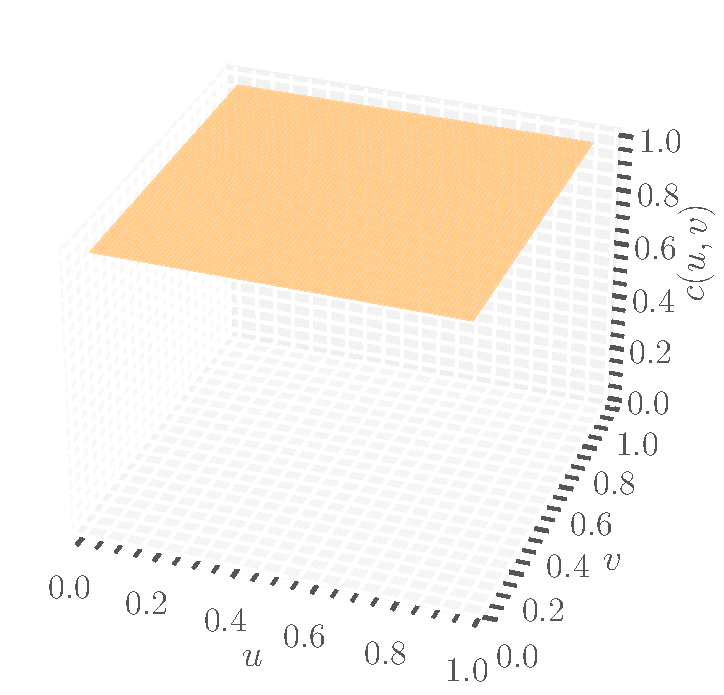
\includegraphics[width=0.4\linewidth]{01_IndependenceCopula_density}
	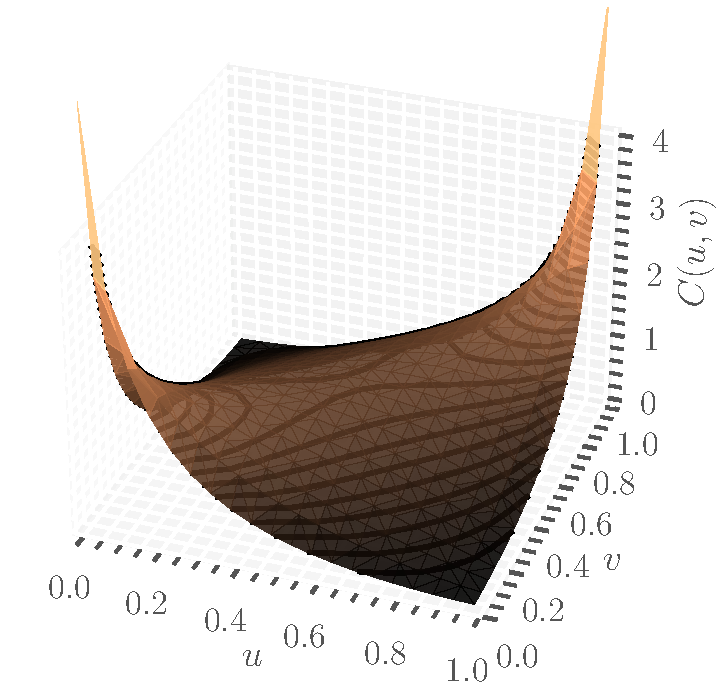
\includegraphics[width=0.4\linewidth]{01_GaussianCopula_density}
	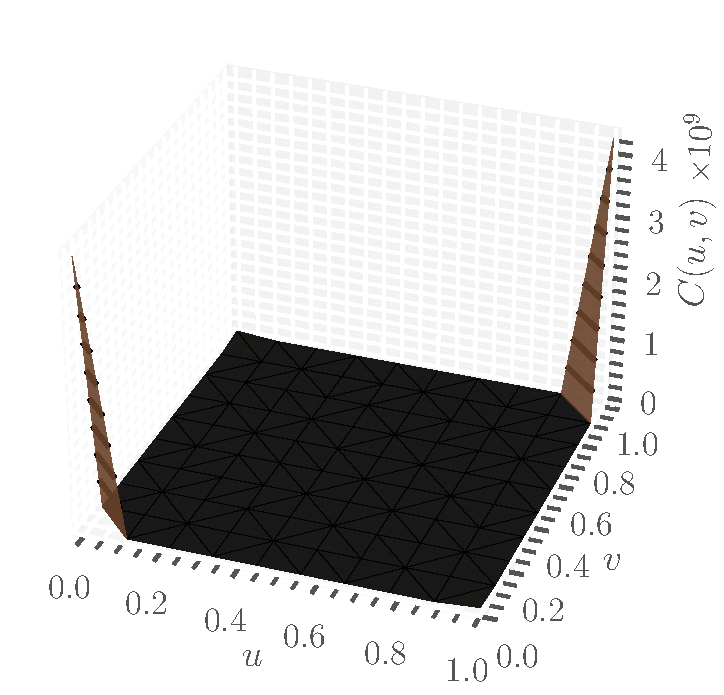
\includegraphics[width=0.4\linewidth]{01_StudentCopula_density}
	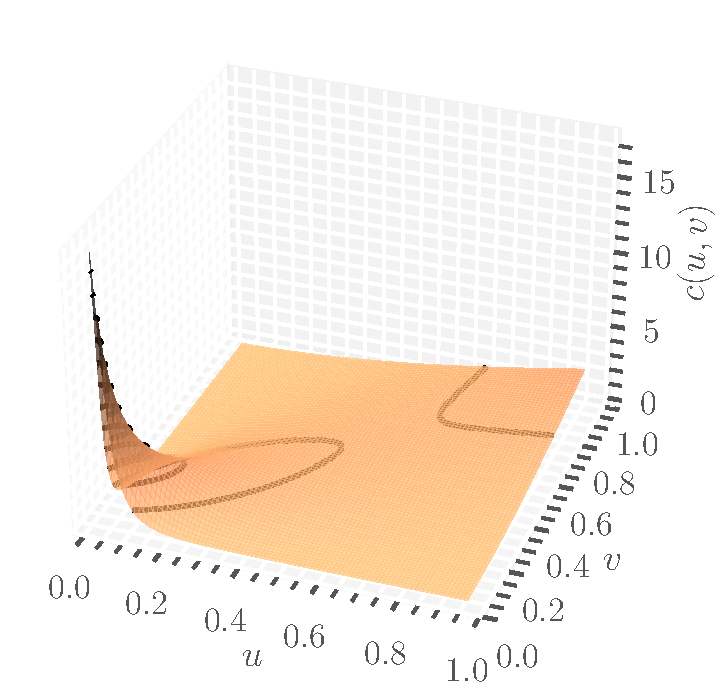
\includegraphics[width=0.4\linewidth]{01_ClaytonCopula_density}
	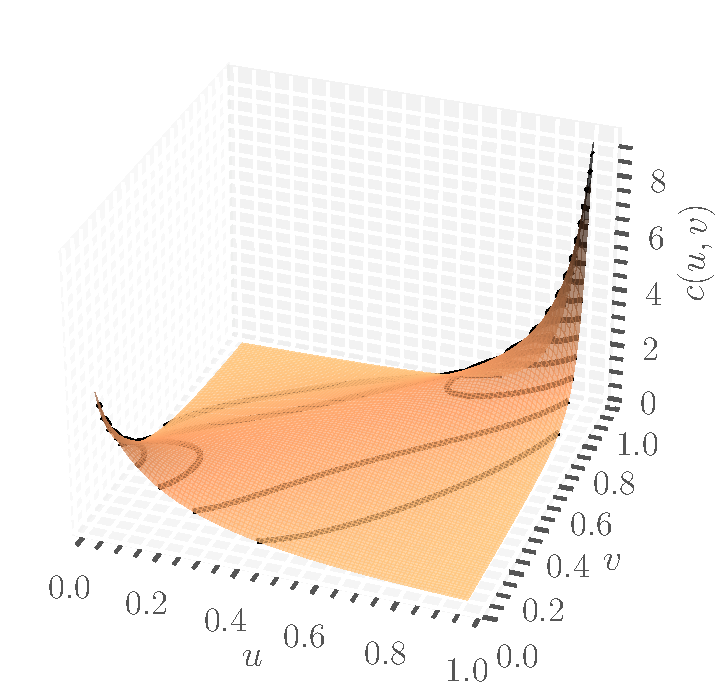
\includegraphics[width=0.4\linewidth]{01_GumbelCopula_density}
	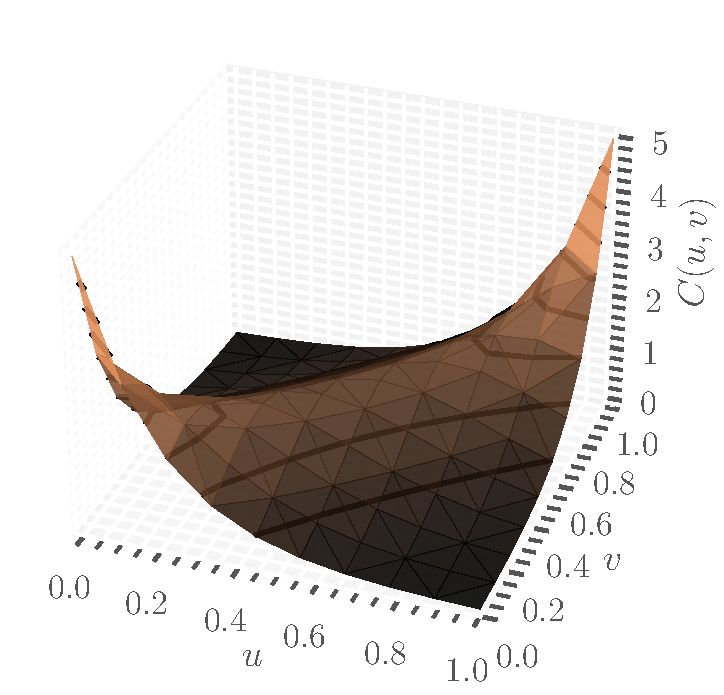
\includegraphics[width=0.4\linewidth]{01_FrankCopula_density}
	
	\caption{Gęstości wybranych kopuł.\label{fig:copula_densities}}
\end{figure}

\label{subsec:dwuwymiarowe_kopuly_przyklady}



\section{Kopuły w wyższych wymiarach}
\label{sec:kopuly_w_wyzszych_wymiarach}

		
\mgrclosechapter